\chapter{Thermal-SZ Weak Lensing Cross Correlation}
\label{cross_correlation}
Once the tSZ maps are found using the above method, we cross-correlate the the tangential
shear component using the Weak-Lensing datasets available.
We compute the cross correlation using
the k-D trees algorithm. k-D trees perform efficiently in nearest neighbour searches and help
speedup calculating the correlation functions significantly. We use the \texttt{treecorr} library
for this \cite{treecorr}. We perform the cross correlation
using the  Red Cluster Sequence Lensing Survey (RCSLens) dataset \cite{rcslens}
and the Planck tSZ skymaps \cite{plancksz}, initially, to verify our cross correlations by
comparing the results with \cite{tszrcscross}.
We repeat the same with the Kilo Degree Survey (KiDS) dataset and
our own tSZ skymaps. 

Following this, we will compare with different theoretical predictions will help us
constrain the cosmology and baryon models. Especially, We are interested in looking at
non-gravitational feedback.

\section{Space Partitioning for quick computation of Correlation functions}
In order to compute the correlation function, We need know the nearest neighbours of every galaxy. Computationally, Looping over all the
galaxies and computing the pairwise distance is a very costly. We would need an algorithm, which lets us know the nearest neighbour without
explicitly computing the distances. There is a class of algorithms, which help us do this; called \emph{Space Partitioning Algorithms}.
\\
Space partitioning systems are often hierarchical, where the algorithm is applied recursively in order to partition the regions. These regions are in general
stored in the form of a \emph{Tree}\footnote{A Tree is a data structure, which is defined recursively, where the values are stored as a collection of nodes, each
  with a root value and also acts as a parent for a sub-tree, represented by a collection of linked nodes}. Finally when the recursion stops at the individual
points instead of regions. These end points of the \emph{tree} are known as \emph{leaves}.
We would specifically be interested in an algorithm called k-D Trees. \\

\subsection{k-D Trees}
k-D trees is a space partitioning data structure,
which constructs the tree based on the proximity of the points without explicitly computing the distances between
the points. k-D Trees are a special case of space partitioning, called binary space partitioning, where each region is divided
into two regions recursively. This also implies, that each node in the \emph{tree} we are constructing will be connected to two other nodes.
\\
In this structure, each leaf-node will be a point from the given data. Each non-leaf-node, will also implicitly divide the space with a
hyper plane, which is parallel to the axis and passes through the point corresponding to the space.

The Algorithm goes as follows,
\begin{enumerate}
\item Choose the median point along a particular axis, and make that into a parent node.
\item Create 2 regions, based on the hyperplane which divides the same axis along the median point.
\item Create two sub-trees for these two regions, and repeat from step 1, while cycling though all possible axis for the choice of axis.
\end{enumerate}

\begin{figure}[H]
  \centering
  \includegraphics[width=0.3\linewidth]{kdtree_2d.png}
  \includegraphics[width=0.3\linewidth]{tree_2d.png}
  \caption{Example k-D Trees partitioning and data structure}
\end{figure}
Finding the nearest neighbours then becomes merely the act of traversing the trees. This immensely speeds
up the computation of correlation functions. 


\subsection{Finding the nearest neighbour}
By efficiently, utilizing the properties of the tree. Nearest Neighbour (NN) search can be done efficiently by quickly eliminating
large chunks of data. The process of searching for nearest neighbours is analogous to the process of searching for particular value on the tree.
This involves traversing the tree starting from the root, and choosing the branch at every node. Since, in the case of a binary  tree. This involves ignoring
the other branch altogether, We can ignore huge chunks of data, without explicitly comparing with the current neighbours. 

The Algorithm goes as follows, 
\begin{enumerate}
\item Start from the root-node of the tree.
\item Compute the distance to the node. Store this value as the best value.
\item Compute the distances to all the children nodes. If any of the values is lesser than the best value. Choose this node and repeat step 2.
\item Exit the Loop when all the children's distances are greater than the best value, or if you reach the leaves of the tree.
\end{enumerate}
If instead of searching for the nearest neighbour, We want all the neighbours till a particular distance. We can also exit the loop once that particular
distance is reached and return all the nodes, belonging to a particular node all the way to the leaves.


\subsection{Ball - Trees}
Ball Tree is a variant of the k-D Trees data structure, where each node is partitions the data into two disjoint sets each associated with a different
hypersphere. Each node in this tree defines the smallest ball, which contains all the data points in it's subtree. The algorithm for construction and searching
for nearest neighbour is similar to the k-d trees algorithm. 
\begin{figure}[htbp]
  \centering
  \includegraphics[width=0.5\linewidth]{ball_trees.png}
  \caption{Ball Trees: a) Initial Hyper-balls (These initializations can be overlapping, but it is made sure that each
    hypersphere contains only one point; It's center)
    b \& c) Ball-Tree structure constructed for the available data (Image Courtesy: \cite{balltree})}
\end{figure}
We use a Python library (\texttt{treecorr}) which computes two point correlation functions, by implementing the ball-tree algorithm. \cite{treecorr}.


\section{Calculation from Data}
\subsection{Observational Data and Sampling}
\subsubsection{Weak Lensing Surveys}
The Data is acquired form the The Red Sequence Cluster survey.
\cite{rcslens}. Their Data is acquired from a MegaCAM camera from
14 seperate patches in the sky with each ranging from
$20$ to $200 \deg^2$. The total survey covers an area of $785\deg^2$ in the sky.
\\
We use cosmic shear measurements from the Kilo-Degree Survey
\cite{kids1, kids2, kids3}, hereafter referred to as KiDS. KiDS is an 
ongoing survey which will eventually cover an area of $1350\deg^2$. 
\comment{Cite theli pre-processing}


\subsubsection{tSZ Skymaps}
For the tSZ skymaps, We use the maps generated by us as explained in the 
previous chapter and also the skymaps provided in the Planck 2015 Public 
Data Release \cite{plancksz}. Since tSZ skymaps are all skymaps, We use 
the entire skymap to compute the correlation function in order to provide 
a large correlation area around the RCSLens fields, which reduces the statistical 
noise. 


\subsubsection{Sampling}
We compute the correlation function separately for each of the 14 RCSLens fields or 4 KiDS fields. We then create jackknife samples of these results 
and them compute the mean and the standard deviation of these samples.

\subsection{Two Point Correlation Functions}
Now, In order to compute the two-point correlation functions 
we work in the configuration space.
For $y-\gamma_T$, we compute the two point correlation function as, 
\begin{align}
  \begin{split}
    \xi^{y - \gamma_T}(\theta) = \frac{\sum\limits_{ij} y^i e^{ij}_t w^j \Delta_{ij}(\theta)}{\sum\limits_{ij} w^j \Delta_{ij}(\theta)}
  \end{split}
\end{align}

where, $y^i$ is the y-value from the tSZ maps in pixel i. And $e^{ij}$ is the tangential ellipticity of the galaxy j in the catalogue with
respect to pixel i. The tangential ellipticity is corrected for both multiplicative and additive bias. $\Delta_{ij}(\theta)$ imposes our binning scheme.
It is one if the angular seperation between i and j is $\theta$ and zero otherwise, and $w^j$ is the \emph{lensfit} weight
(For definition see Reference \cite{weightdef}). 

\subsection{Bias Correction}
During the measurement of the ellipticities there exists calibration corrections to account for biases in our measurement. These are modelled by a
multiplicative term and an additive term such that,

\begin{align}
  \begin{split}
    g^{obs}_i = (1 + m)g^{true}_i + c
  \end{split}
\end{align}

Estimates of these biases from image simulations are given to us as part of the catalogue and we need to correct for them before computing the correlation
functions. The RCSLens catalogue contains two additive biases, Detector Bias and Noise Bias, whereas the KiDS catalogue contains only a multiplicative bias which
needs to be corrected for. More information can be found in the respective catalogue information. 



\subsection{Systematic Tests}
In order to test for systematics in the data, We perform 2 systematic tests.
\begin{itemize}
\item \textbf{We calculate $\langle y \gamma_x \rangle$}: We can compute this by rotating the sources by $45^\circ$ (ie, $e_{1,new} = e_{2,old}$ and
  $e_{2,new} = -e_{1,old}$. We saw in a previous section how this will always be zero for spherically symmetric mass distributions \ref{weaklensing}.

\item \textbf{We randomise the catalogue and find the correlation once again}: Since the catalogues are randomized (un-correlated),
  The correlation functions will become zero.
  Any deviations from zero, will show the existence of biases in our methodology.
\end{itemize}
in the absence of systematic errors, in our calculation. Both of these tests should give us values close to zero.

\section{Results}
Now, Computing the cross-correlation using the Planck SkyMaps and our own sky maps, We get the following results.
\begin{figure}[H]
  \centering
  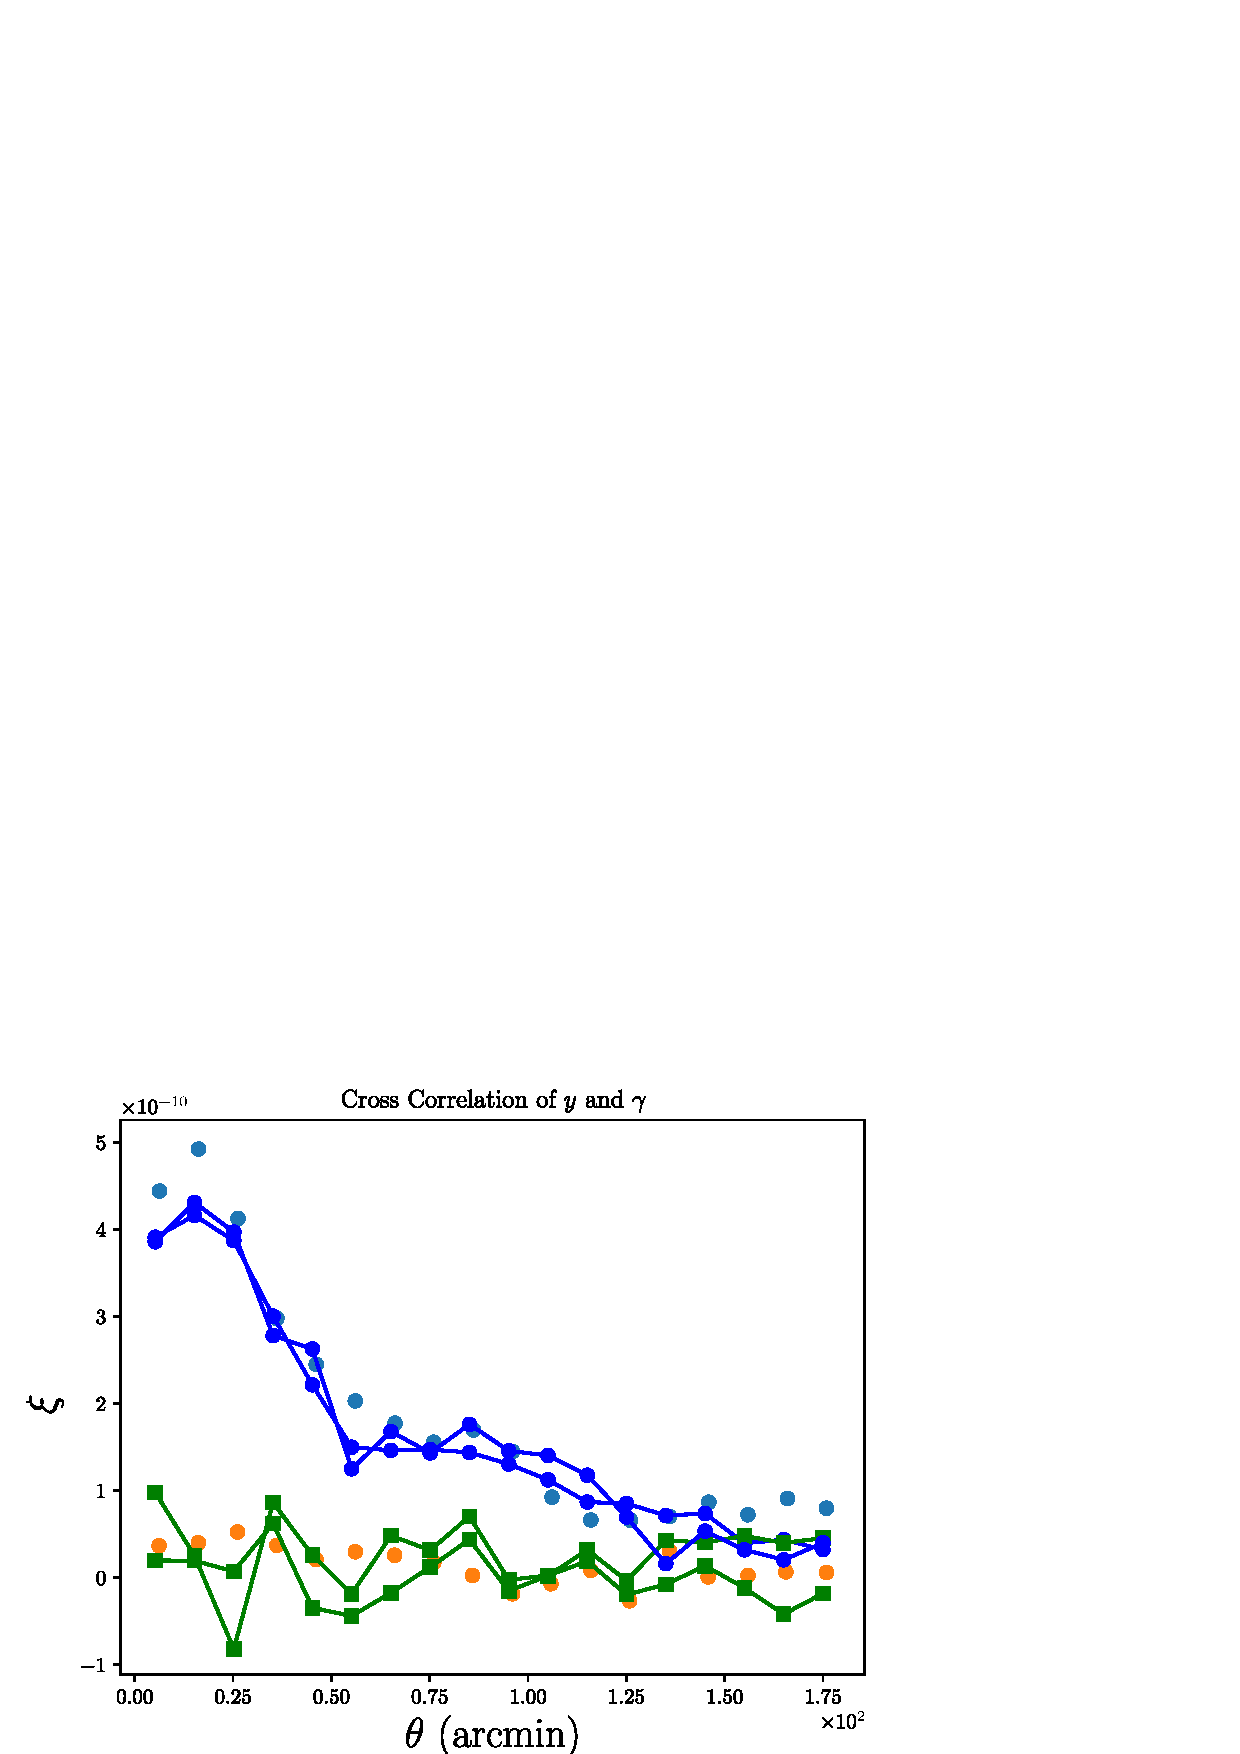
\includegraphics[width=0.7\linewidth]{plot_rcs.pdf}
  \caption{Cross Correlation between tSZ and Weak Lensing maps for RCSLens fields}
\end{figure}

\begin{figure}[H]
  \centering
  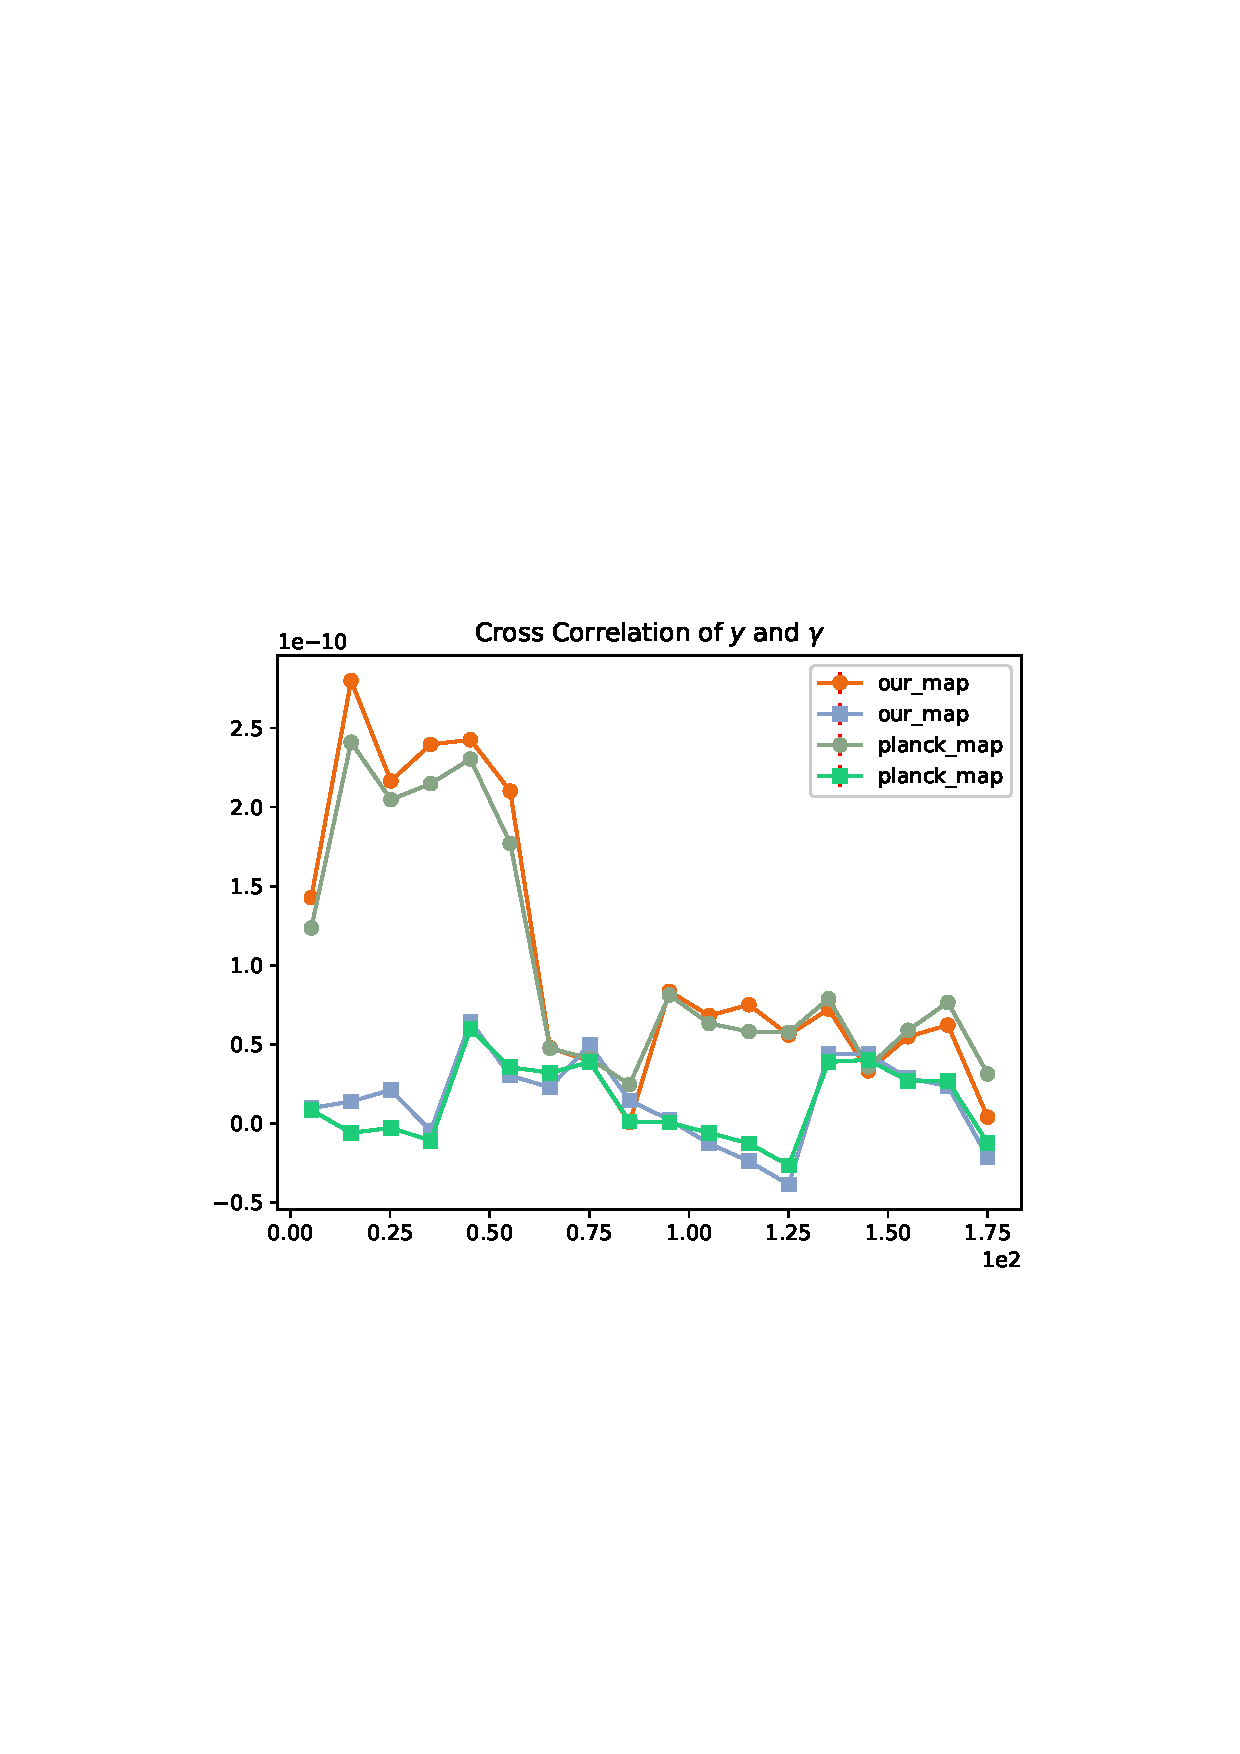
\includegraphics[width=0.7\linewidth]{plot_kids.pdf}
  \caption{Cross Correlation between tSZ and Weak Lensing maps for KiDs fields}
\end{figure}


\section{Comparison with Theory}
\label{theory}
We like to compare our observations with theoretical predicitions based on Halo models, closely
following the method developed by 
\cite{halotheoryma}. Currently we are concentrating on computing the real space cross correlation
$ \xi = \langle \gamma_T - y \rangle$ , By using
\begin{equation}
  \label{realcrosstheory}
  \xi^{y - \gamma_T} (\theta) = \int \frac{d^2 \vec{l}}{2\pi^2 } C_l^{y-k} \cos(2(\phi - \psi)) \exp(i \theta \cos(\phi - \psi))
\end{equation}
Where, $\phi$ is the Polar angle with respect to the coordinate system and $\psi$ is the angle
between $\vec{l}$ and the coordinate.

In order to compute the $y - k$ cross correlation power spectra found in Equation
\ref{realcrosstheory}, we use the 1-halo term as defined in \cite{haloreview}.
\begin{equation}
  C_l^{y-k,1h} = \int\limits_0^{z_{max}} dz \frac{dV}{dz d\Omega} \int\limits_{M_{min}}^{M_{max}} dM \frac{dn}{dM} y_l (M, z) k_l (M,z)
\end{equation}
For the halo mass function, We use the form suggested by Sheth and Tormen \cite{massfunctionsheth}
For the convergence profile in fourier space, We use
\begin{equation}
  k_l = \frac{W^k(z)}{\xi^2(z)} \frac{1}{\rho_m} 4 \pi \int\limits_0 ^{r_{vir}} dr r^2 \frac{\sin(lr/\xi)}{lr/\xi} \rho(r;M,z)
\end{equation}
   \\
And for the fourier transform of the projected gas pressure.
\begin{equation}
    y_l = \frac{4 \pi r_s}{l^2_s} \frac{\sigma_T}{m_e c^2} \int dx x^2  \frac{\sin(lx/\xi)}{lx/\xi} P_e(x;M,z)
\end{equation}
\\
For electron pressure, We use the \emph{universal pressure profile} and the NFW model. 
We plan to use the best fit parameters for the Pressure profile from the Planck Collaboration
and then compare the halo model predictions from both the Planck and WMAP-7yr cosmologies. To look
for any non-gravitational feedback, we plan to use the method developed by \cite{subhapaper},
applied to tSZ $C_l$s.


%%% Local Variables:
%%% mode: latex
%%% TeX-master: "thesis"
%%% End:
